Consider the following sequence of calls:

\texttt{init(7, [10, 20, 60, 40, 50, 30, 70])}


\texttt{max\_towers(1, 5, 10)}

Pak Dengklek can lease towers $1$, $3$, and $5$.
The example is illustrated in the following picture, where shaded trapezoids represent leased towers.

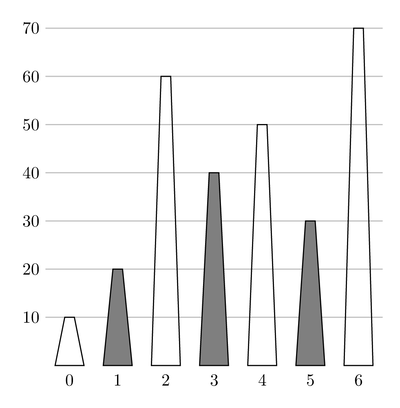
\includegraphics{towers-example.png}

Towers $3$ and $5$ can communicate using tower $4$ as an intermediary, since $40 \le 50 - 10$ and $30 \le 50 - 10$.
Towers $1$ and $3$ can communicate using tower $2$ as an intermediary.
Towers $1$ and $5$ can communicate using tower $3$ as an intermediary.
There is no way to lease more than $3$ towers, therefore the procedure should return $3$.

\texttt{max_towers(2, 2, 100)}

There is only $1$ tower in the range, thus Pak Dengklek can only lease $1$ tower.
Therefore the procedure should return $1$.

\texttt{max\_towers(0, 6, 17)}  

Pak Dengklek can lease towers $1$ and $3$.
Towers $1$ and $3$ can communicate using tower $2$ as an intermediary, since $20 \le 60 - 17$ and $40 \le 60 - 17$.
There is no way to lease more than $2$ towers, therefore the procedure should return $2$.

